\chapter{Možnosti rozšírenia}
V tejto kapitole sa pozrieme na rôzne možnosti a smery, akými by sme mohli našu aplikáciu ďalej rozšíriť.
\section{Ukladanie výstupu do súboru}
Niektoré analyzátory ponúkajú ukladanie výpisu do rôznych súborov. V prípade ak by sme sa rozhodli našu aplikáciu rozšíriť o možnosť ukladania analýzy do súboru, museli by sme si rozmyslieť niekoľko nasledujúcich vecí:

\paragraph{Formát výpisu}
\hfill \break
Akým spôsobom bude vyzerať výstup analýzy. Na výber máme viacero možností od obyčajného textového výstupu až po obrázky alebo rôzne tabuľky. Na začiatok by nebolo príliš zložité zaintegrovať výpis analýzy v textovom formáte. Všetky dáta máme interne reprezentované v podobe QByteArray alebo stromovej štruktúry, ktoré je možné jednoducho prechádzať. Samozrejme musíme myslieť na to, že textový výpis nie je tak flexibilný a interaktívny ako prípadný QTreeView, takže vyobrazenie stromovej štruktúry by pravdepodobne nevyzeralo ideálne.

\paragraph{Rozhodnutie užívateľa, či bude danú analýzu ukladať do súboru alebo nie}
\hfill \break
Musíme myslieť na to, v akej fáze programu umožníme užívateľovi sa najneskôr rozhodnúť o ukladaní danej analýzy do súboru. Momentálne si všetky dáta uchovávame v samostatných QTableWidgetItemoch uložených v QTableWidgete hlavného okna aplikácie. Užívateľ má ale možnosť toto okno \uv{vyčistiť} pomocou tlačidla Clear~\ref{kap04:sec:clear_button}, ktoré vymaže všetky QTableWidgetItemy a tým pádom stratíme referenciu na všetky dáta, ktoré v sebe dané itemy uchovávajú. Doteraz sme sa tým nemuseli zaoberať, pretože dané dáta sem potrebovali na analýzu paketov reprezentovaných riadkom v QTableWidgete, takže akonáhle bol riadok vymazaný pomocu Clear tlačidla, detailnejšia analýza daného paketu už nebola možná. Niektoré možné riešenia tohto problému by mohli byť nasledujúce:
\begin{itemize}
\item V prípade, že umožníme užívateľovi si uložiť analýzu do súboru len do momentu pokiaľ nestlačí tlačidlo Start, máme na výber prakticky 2 možnosti:
\begin{enumerate}
\item \label{kap05:sec:refer} Ukladať si referencie na jednotlivé QTableWidgetItemy až do momentu skončenia programu, kedy jednorázovo zapíšeme do súboru celú analýzu.
\item \label{kap05:sec:priebez} Priebežne zapisovať do súboru analýzu jednotlivých paketov.
\end{enumerate}
Riešenie~\ref{kap05:sec:refer} prináša tú nevýhodu, že si musíme držať v pamäti všetky dáta paketov a zároveň by ukončenie aplikácie trvalo dlhšiu dobu, pretože by sa musela postupne vykonať a zapísať detailná analýza každého paketu. Naopak riešenie~\ref{kap05:sec:priebez} nás zbavuje oboch týchto problémov, ale mohla by mať nepriaznivý dopad na užívateľskú interakciu s aplikáciou, pretože v pozadí by prebiehal proces zapisovania a analýzy. To by sa samozrejme dalo optimalizovať rôznymi spôsobmi -- zapisovať len v momente pokiaľ užívateľ neinteraguje s aplikáciou, využiť metódy paralelného programovania a na zápis/analýzu použiť viac vláken, atď.

\item V prípade, že umožníme užívateľovi rozhodnúť o zápise do súboru hocikedy v priebehu používania aplikácie, musíme mať dáta jednotlivých paketov k dispozícii aj po ich odstráneni z QTableWidgetu tlačidlom Clear. Ako toho dosiahnuť sme naznačili vyššie v riešení~\ref{kap05:sec:refer} spolu s jeho nevýhodami.
\end{itemize}

Dôležité je ale spomenúť, že pridaním ukladania výpisu do súboru nijakým vážnym spôsobom nezasahujeme do programu a nemodifikujeme už naimplementované časti. Všetky dáta máme v aplikácii pripravené a jediné čo nám ostáva vyriešiť je ich spracovanie do súboru.

\section{Iná vizuálna reprezentácia dát}
Momentálne vyobrazujeme dáta za pomoci viewerov -- QTableView, QTreeView. Ako sme si už spomínali vyššie, celé to prebieha na základe Model/View architektúry, ktorá nám umožnuje od seba oddeliť dáta a spôsob akým ich vyobrazujeme. Na základe toho by pre nás nemalo byť tak náročné implementovať nové spôsoby vizuálnej reprezentácie dát. To by sme vedeli dosiahnuť pridaním nového typu vieweru. Mohli by sme si vybrať z už existujúcich, alebo si kľudne naimplementovať vlastný, ktorý by odpovedal našim predstavám vyobrazenia dát. Momentálne máme vytvorených viacero modelov pre špecifické časti našich dát (HexdumpModel pre všetky dáta paketu na vyobrazenie hexdumpu, USBPCapHeaderModel pre hlavičku paketu na jej vyobrazenie pomocou stromovej štruktúry, atď.). Všetky tieto modely sme implementovali z dôvodu aby sme jednoducho vedeli vyobraziť dáta v jednotlivých vieweroch. Preto by pridanie nového vieweru malo pravdepodobne za následok nutnosť implementovať aj tomu odpovedajúci model.

Zaujímavý spôsob vyobrazenia dát by bolo napríklad pomocou koláčového grafu. Vedeli by sme tak vizuálne zobraziť pomer rôznych dát ako napríklad:
\begin{itemize}
\item pomer rôznych typov prenosov (Control/Interrupt/Bulk/Isochronous) počas zachytávania paketov.
\item pomer veľkosti dát hlavičky paketu a zvyškových dát.
\item pomer veľkosti dát poslaných zariadením a USB hostom.
\item pomer zvyškových dát v paketoch vzhľadom na typ prenosu. 
\end{itemize}

Takisto by mohlo byť zaujímavé vyobraziť dáta viac grafickým spôsobom, napríklad ako je ukázané na obrázku~\ref{obr:kap5:graphics_packets} nižšie.

\begin{figure}[!htb]
	\centering
	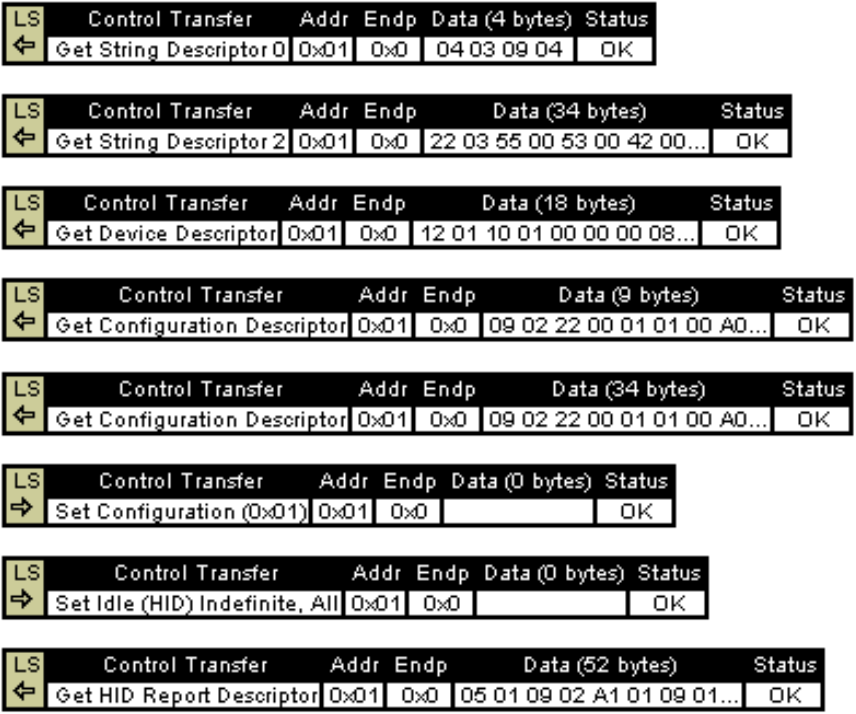
\includegraphics[width=12cm]{img/kap05_graphics_packets}
	\caption{Ukážka grafického vyobrazenia paketov. Obrázok prevzatý zo stránky USB Made Simple~\cite{usbmadesimple_graphics}}
	\label{obr:kap5:graphics_packets}
\end{figure}

\newpage
\section{Pridávanie nových interpreterov pre descriptory}
pridanie nových druhov descriptorov - pridať nový interpreter do factory
\section{Pridanie intepreteru na interrupt tranfser}
pridanie analyzy interrupt transferu aj pre ine ako hid zariadenia
\subsection{Pridanie nových HID zariední}
nove HID zariadenie - pridanie do interrupt ''factory''
\section{Pridanie analýzy pre isochronous a bulk transfer}
semanticka analyza aj inych ako interrupt alebo control transferov - momentalne su rozpoznavane len v hexdumpe
\section{?Možnosť rozšírenia na iné platformy?}
uprava aplikacie aby bola prenositelna aj na ine platformy, co vsetko by tam bolo treba upravit(pravdepodobne nie vela, kedze qt je prenosne, a prakticky jedine co pouzivam spojene s windowsom su jeho structy na rozne descriptory)
